
\documentclass{article}
\usepackage{amsmath}
\usepackage{fancyhdr}
\usepackage{titling}
\usepackage{graphicx}
\usepackage{tcolorbox}
\usepackage{float} % for [H] specifier

% Define your information
\newcommand{\classname}{MATH 412}
\newcommand{\assignmentname}{Project 1}

% Define fancyhdr style for header
\pagestyle{fancy}
\fancyhf{} % Clear header and footer
\fancyhead[L]{\myname} % Your name in upper left corner
\fancyhead[C]{\classname} % Class name in upper middle
\fancyhead[R]{\assignmentname} % Assignment name in upper right corner
\renewcommand{\headrulewidth}{0.4pt} % Header line width

\begin{document}

\title{MATH 412 - Project 1}
\author{Erica Cain, Takiya Eastmond, Makayla Greer, Twymun Safford}
\date{February 20th, 2024}

\begin{titlingpage}
    \begin{center}
        \vspace*{3cm}
        {\Huge \thetitle}\\[0.5cm]
        {\Large \theauthor}\\[2cm]
        {\large \thedate}
    \end{center}
\end{titlingpage}

% Set page numbering style to arabic (1, 2, 3, ...)
\pagenumbering{arabic}

% Define footer style for pages with page numbers at the bottom
\fancyfoot[C]{\thepage}

\title{Computer Graphics - Project I}
\author{Erica Cain, Takiya Eastmond, Makayla Greer, Twymun Safford}
\date{February 20th, 2024}

\begin{titlingpage}
    \begin{center}
        \vspace*{3cm}
        {\Huge \thetitle}\\[0.5cm]
        {\Large \theauthor}\\[2cm]
        {\large \thedate}
    \end{center}
\end{titlingpage}

\section*{Projects 1 - Computer Graphics I}

\subsection*{Problem 1}

Apply each of the three transformations given in Table 1 to these vertices and sketch the result, to verify that each transformation has the indicated effect. Use $c=2$ in the expansion matrix and in the shear
matrix.

\subsubsection*{Reflection Matrix}

The points of the grey square as depicted below:

\begin{figure}[!htb]
  \centering
  \includegraphics[width=0.45\textwidth]{grey_square.PNG}
  \label{fig3}
\end{figure}

Can be expressed as:

\[P = 
\begin{bmatrix}
    0 & 1 & 1 & 0 \\
    0 & 0 & 1 & 1 \\
\end{bmatrix}
\]

The reflection matrix is:

\[T_{1} = 
\begin{bmatrix}
    1 & 0  \\
    0 & -1  \\
\end{bmatrix}
\]

Acting with matrix $T_1$ on matrix $P$ yields:

\[ 
P' = T1 \cdot P = \begin{bmatrix}
t_{11} & t_{12} \\
t_{21} & t_{22} \\
\end{bmatrix} \cdot \begin{bmatrix}
p_{11} & p_{12} & p_{13} & p_{14} \\
p_{21} & p_{22} & p_{23} & p_{24} \\
\end{bmatrix}
\]
\[P' =  
\begin{bmatrix}
    t_{11}p_{11} + t_{12}p_{21} & t_{11}p_{12} + t_{12}p_{22} & t_{11}p_{13} + t_{12}p_{23} & t_{11}p_{14} + t_{12}p_{24} \\
    t_{21}p_{11} + t_{22}p_{21} & t_{21}p_{12} + t_{22}p_{22} & t_{21}p_{13} + t_{22}p_{23} & t_{21}p_{14} + t_{22}p_{24}
\end{bmatrix}
\]

\[P' = 
\begin{bmatrix}
    0 & 1 & 1 & 0 \\
    0 & 0 & -1 & -1 \\
\end{bmatrix}
\]

Which corresponds to a reflection across the x-axis. This is depicted in graph:

\begin{figure}
  \centering
  \includegraphics[width=0.6\textwidth]{problem1a_figure.PNG}
  \label{fig3}
\end{figure}

\subsubsection*{Expansion/Contraction Matrix}

The points of the grey square as depicted below:

\begin{figure}[!htb]
  \centering
  \includegraphics[width=0.45\textwidth]{grey_square.PNG}
  \label{fig3}
\end{figure}

Can be expressed as:

\[P = 
\begin{bmatrix}
    0 & 1 & 1 & 0 \\
    0 & 0 & 1 & 1 \\
\end{bmatrix}
\]

The expansion matrix is:

\[T_{2} = 
\begin{bmatrix}
    2 & 0  \\
    0 & 1  \\
\end{bmatrix}
\]

Acting with matrix $T_2$ on matrix $P$ yields:

\[ 
P' = T2 \cdot P = \begin{bmatrix}
t_{11} & t_{12} \\
t_{21} & t_{22} \\
\end{bmatrix} \cdot \begin{bmatrix}
p_{11} & p_{12} & p_{13} & p_{14} \\
p_{21} & p_{22} & p_{23} & p_{24} \\
\end{bmatrix}
\]
\[P' =  
\begin{bmatrix}
    t_{11}p_{11} + t_{12}p_{21} & t_{11}p_{12} + t_{12}p_{22} & t_{11}p_{13} + t_{12}p_{23} & t_{11}p_{14} + t_{12}p_{24} \\
    t_{21}p_{11} + t_{22}p_{21} & t_{21}p_{12} + t_{22}p_{22} & t_{21}p_{13} + t_{22}p_{23} & t_{21}p_{14} + t_{22}p_{24}
\end{bmatrix}
\]

\[P' = 
\begin{bmatrix}
    0 & 2 & 2 & 0 \\
    0 & 0 & 1 & 1 \\
\end{bmatrix}
\]

Which corresponds to increasing the horizontal dimension of the square by a factor of 2. This is depicted in graph:

\begin{figure}[!htb]
  \centering
  \includegraphics[width=0.6\textwidth]{problem1b_figure.PNG}
  \label{fig3}
\end{figure}

\subsubsection*{Shear Matrix}

The points of the grey square as depicted below:

\begin{figure}[!htb]
  \centering
  \includegraphics[width=0.45\textwidth]{grey_square.PNG}
  \label{fig3}
\end{figure}

Can be expressed as:

\[P = 
\begin{bmatrix}
    0 & 1 & 1 & 0 \\
    0 & 0 & 1 & 1 \\
\end{bmatrix}
\]

The shear matrix is:

\[T_{3} = 
\begin{bmatrix}
    1 & 1  \\
    0 & 1  \\
\end{bmatrix}
\]

Acting with matrix $T_3$ on matrix $P$ yields:

\[ 
P' = T3 \cdot P = \begin{bmatrix}
t_{11} & t_{12} \\
t_{21} & t_{22} \\
\end{bmatrix} \cdot \begin{bmatrix}
p_{11} & p_{12} & p_{13} & p_{14} \\
p_{21} & p_{22} & p_{23} & p_{24} \\
\end{bmatrix}
\]
\[P' =  
\begin{bmatrix}
    t_{11}p_{11} + t_{12}p_{21} & t_{11}p_{12} + t_{12}p_{22} & t_{11}p_{13} + t_{12}p_{23} & t_{11}p_{14} + t_{12}p_{24} \\
    t_{21}p_{11} + t_{22}p_{21} & t_{21}p_{12} + t_{22}p_{22} & t_{21}p_{13} + t_{22}p_{23} & t_{21}p_{14} + t_{22}p_{24}
\end{bmatrix}
\]

\[P' = 
\begin{bmatrix}
    0 & 1 & 2 & 1 \\
    0 & 0 & 1 & 1 \\
\end{bmatrix}
\]

Which corresponds to a shear in the x-direction by a factor of 1. This is depicted in the graph below:

\begin{figure}[!htb]
  \centering
  \includegraphics[width=0.6\textwidth]{problem1c_figure.PNG}
  \label{fig3}
\end{figure}


\subsection*{Problem 2}

Verify that multiplication by the given matrix has the indicated effect when applied to the gray square in the
table. Use $c=3$ in the expansion matrix and $c=1$ in the shear matrix.

\subsubsection*{Reflection Matrix}

The points of the grey square as depicted below:

\begin{figure}[!htb]
  \centering
  \includegraphics[width=0.45\textwidth]{grey_square.PNG}
  \label{fig3}
\end{figure}

Can be expressed as:

\[P = 
\begin{bmatrix}
    0 & 1 & 1 & 0 \\
    0 & 0 & 1 & 1 \\
\end{bmatrix}
\]

The reflection matrix is:

\[T_{1} = 
\begin{bmatrix}
    -1 & 0  \\
    0 & 1  \\
\end{bmatrix}
\]

Acting with matrix $T_1$ on matrix $P$ yields:

\[ 
P' = T1 \cdot P = \begin{bmatrix}
t_{11} & t_{12} \\
t_{21} & t_{22} \\
\end{bmatrix} \cdot \begin{bmatrix}
p_{11} & p_{12} & p_{13} & p_{14} \\
p_{21} & p_{22} & p_{23} & p_{24} \\
\end{bmatrix}
\]
\[P' =  
\begin{bmatrix}
    t_{11}p_{11} + t_{12}p_{21} & t_{11}p_{12} + t_{12}p_{22} & t_{11}p_{13} + t_{12}p_{23} & t_{11}p_{14} + t_{12}p_{24} \\
    t_{21}p_{11} + t_{22}p_{21} & t_{21}p_{12} + t_{22}p_{22} & t_{21}p_{13} + t_{22}p_{23} & t_{21}p_{14} + t_{22}p_{24}
\end{bmatrix}
\]

\[P' = 
\begin{bmatrix}
    0 & 1 & 1 & 0 \\
    0 & 0 & -1 & -1 \\
\end{bmatrix}
\]

Which corresponds to a reflection across the y-axis. This is depicted in graph as the red square (the blue square is the original square):

\begin{figure}[!htb]
  \centering
  \includegraphics[width=0.6\textwidth]{problem2a.PNG}
  \label{fig3}
\end{figure}

\subsubsection*{Expansion/Contraction Matrix}

The points of the grey square as depicted below:

\begin{figure}[!htb]
  \centering
  \includegraphics[width=0.45\textwidth]{grey_square.PNG}
  \label{fig3}
\end{figure}

Can be expressed as:

\[P = 
\begin{bmatrix}
    0 & 1 & 1 & 0 \\
    0 & 0 & 1 & 1 \\
\end{bmatrix}
\]

The expansion matrix is:

\[T_{2} = 
\begin{bmatrix}
    1 & 0  \\
    0 & 3  \\
\end{bmatrix}
\]

Acting with matrix $T_2$ on matrix $P$ yields:

\[ 
P' = T1 \cdot P = \begin{bmatrix}
t_{11} & t_{12} \\
t_{21} & t_{22} \\
\end{bmatrix} \cdot \begin{bmatrix}
p_{11} & p_{12} & p_{13} & p_{14} \\
p_{21} & p_{22} & p_{23} & p_{24} \\
\end{bmatrix}
\]
\[P' =  
\begin{bmatrix}
    t_{11}p_{11} + t_{12}p_{21} & t_{11}p_{12} + t_{12}p_{22} & t_{11}p_{13} + t_{12}p_{23} & t_{11}p_{14} + t_{12}p_{24} \\
    t_{21}p_{11} + t_{22}p_{21} & t_{21}p_{12} + t_{22}p_{22} & t_{21}p_{13} + t_{22}p_{23} & t_{21}p_{14} + t_{22}p_{24}
\end{bmatrix}
\]

\[P' = 
\begin{bmatrix}
    0 & 1 & 1 & 0 \\
    0 & 0 & 3 & 3 \\
\end{bmatrix}
\]

Which corresponds to increasing the height of the square (now rectangle) by a factor of 3. This is represented below:

\begin{figure}[H]
  \centering
  \includegraphics[width=0.55\textwidth]{problem2b(2).PNG}
  \label{fig3}
\end{figure}

\subsubsection*{Shear Matrix}

The points of the grey square can be expressed as:

\[P = 
\begin{bmatrix}
    0 & 1 & 1 & 0 \\
    0 & 0 & 1 & 1 \\
\end{bmatrix}
\]

The shear matrix is:

\[T_{3} = 
\begin{bmatrix}
    1 & 0  \\
    1 & 1  \\
\end{bmatrix}
\]

Acting with matrix $T_3$ on matrix $P$ yields:

\[ 
P' = T1 \cdot P = \begin{bmatrix}
t_{11} & t_{12} \\
t_{21} & t_{22} \\
\end{bmatrix} \cdot \begin{bmatrix}
p_{11} & p_{12} & p_{13} & p_{14} \\
p_{21} & p_{22} & p_{23} & p_{24} \\
\end{bmatrix}
\]
\[P' =  
\begin{bmatrix}
    t_{11}p_{11} + t_{12}p_{21} & t_{11}p_{12} + t_{12}p_{22} & t_{11}p_{13} + t_{12}p_{23} & t_{11}p_{14} + t_{12}p_{24} \\
    t_{21}p_{11} + t_{22}p_{21} & t_{21}p_{12} + t_{22}p_{22} & t_{21}p_{13} + t_{22}p_{23} & t_{21}p_{14} + t_{22}p_{24}
\end{bmatrix}
\]

\[P' = 
\begin{bmatrix}
    0 & 1 & 1 & 0 \\
    0 & 1 & 2 & 1 \\
\end{bmatrix}
\]

Which corresponds to a shear in the y-direction by 1. This is represented below:

\begin{figure}[!htb]
  \centering
  \includegraphics[width=0.65\textwidth]{problem2c(3).PNG}
  \label{fig3}
\end{figure}


\subsection*{Problem 3}

Let \[T = 
\begin{bmatrix}
    1 & 1.5  \\
    0 & 1  \\
\end{bmatrix}
\]

\subsubsection*{Part a}

T does an extreme shear on the grey square, P,  - shearing by a factor of 0.5.

\[ 
P' = T \cdot P = \begin{bmatrix}
t_{11} & t_{12} \\
t_{21} & t_{22} \\
\end{bmatrix} \cdot \begin{bmatrix}
p_{11} & p_{12} & p_{13} & p_{14} \\
p_{21} & p_{22} & p_{23} & p_{24} \\
\end{bmatrix}
\]
\[P' =  
\begin{bmatrix}
    t_{11}p_{11} + t_{12}p_{21} & t_{11}p_{12} + t_{12}p_{22} & t_{11}p_{13} + t_{12}p_{23} & t_{11}p_{14} + t_{12}p_{24} \\
    t_{21}p_{11} + t_{22}p_{21} & t_{21}p_{12} + t_{22}p_{22} & t_{21}p_{13} + t_{22}p_{23} & t_{21}p_{14} + t_{22}p_{24}
\end{bmatrix}
\]

\[P' = 
\begin{bmatrix}
    0 & 1 & 2.5 & 1.5 \\
    0 & 0 & 1 & 1 \\
\end{bmatrix}
\]

\subsubsection*{Part b}

Given a matrix $T$, the formula for finding its inverse $T^{-1}$ is:

\begin{equation*}
T^{-1} = \frac{1}{\det(T)} \cdot \text{adj}(T)
\end{equation*}

where $\det(T)$ is the determinant of matrix $T$, and $\text{adj}(T)$ is the adjugate (or adjoint) of $T$.
The $\det(T)$ for a 2 x 2 matrix is $(ad-bc)$. For the matrix T that is $(1*1 - (1.5*0))$ = 1. 
The adjoint, $\text{adj}(T)$, is:

\[adj(T) = 
\begin{bmatrix}
    1 & -1.5  \\
    0 & 1  \\
\end{bmatrix}
\]

Therefore:

\[T^{-1} = 
\begin{bmatrix}
    1 & -1.5  \\
    0 & 1  \\
\end{bmatrix}
\]


\begin{figure}[H]
  \centering
  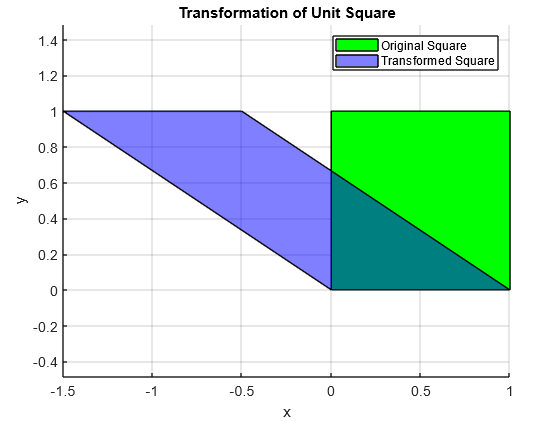
\includegraphics[width=1.00\textwidth]{extreme_shear_left.PNG}
  \label{fig3}
\end{figure}

\subsubsection*{Part c}

$T^{-1}$ does an extreme shear on the grey square, but shearing to the negative direction for x. 

\[ 
P' = T^{-1} \cdot P = \begin{bmatrix}
t_{11} & t_{12} \\
t_{21} & t_{22} \\
\end{bmatrix} \cdot \begin{bmatrix}
p_{11} & p_{12} & p_{13} & p_{14} \\
p_{21} & p_{22} & p_{23} & p_{24} \\
\end{bmatrix}
\]
\[P' =  
\begin{bmatrix}
    t_{11}p_{11} + t_{12}p_{21} & t_{11}p_{12} + t_{12}p_{22} & t_{11}p_{13} + t_{12}p_{23} & t_{11}p_{14} + t_{12}p_{24} \\
    t_{21}p_{11} + t_{22}p_{21} & t_{21}p_{12} + t_{22}p_{22} & t_{21}p_{13} + t_{22}p_{23} & t_{21}p_{14} + t_{22}p_{24}
\end{bmatrix}
\]

\[P' = 
\begin{bmatrix}
    0 & 1 & -0.5 & -1.5 \\
    0 & 0 & 1 & 1 \\
\end{bmatrix}
\]




\subsubsection*{Part d}

Multiplying the matrix $T$ with the matrix $T^{-1}$ should yield the identity matrix:

\[T = 
\begin{bmatrix}
    1 & 1.5  \\
    0 & 1  \\
\end{bmatrix}
\]

\[T^{-1} = 
\begin{bmatrix}
    1 & -1.5  \\
    0 & 1  \\
\end{bmatrix}
\]

\[T^{-1} T = 
\begin{bmatrix}
    1 & 0  \\
    0 & 1  \\
\end{bmatrix}
\]

Therefore, $T^{-1}(T(S))$ should reproduce the same unit square we started with. That is:

\begin{figure}[!htb]
  \centering
  \includegraphics[width=0.45\textwidth]{grey_square.PNG}
  \label{fig3}
\end{figure}

Which expressed as a matrix:

\[S = 
\begin{bmatrix}
    0 & 1 & 1 & 0 \\
    0 & 0 & 1 & 1 \\
\end{bmatrix}
\]

\subsection*{Problem 4}

\subsubsection*{Part a}

Let T be an expansion matrix such that:

Let \[T = 
\begin{bmatrix}
    3 & 0  \\
    0 & 1  \\
\end{bmatrix}
\]

Acting with this expansion matrix on the unit square, S, yields:

\[ 
P' = T \cdot S = 
\begin{bmatrix}
    t_{11}s_{11} + t_{12}s_{21} & t_{11}s_{12} + t_{12}s_{22} & t_{11}s_{13} + t_{12}s_{23} & t_{11}s_{14} + t_{12}s_{24} \\
    t_{21}s_{11} + t_{22}s_{21} & t_{21}s_{12} + t_{22}s_{22} & t_{21}s_{13} + t_{22}s_{23} & t_{21}s_{14} + t_{22}s_{24}
\end{bmatrix}
\]

\[P' = 
\begin{bmatrix}
    0 & 3 & 3 & 0 \\
    0 & 0 & 1 & 1 \\
\end{bmatrix}
\]

This represents an expansion along the horizontal axis for the square by a factor of 3.

\subsubsection*{Part b}

Let S be an expansion matrix such that:

Let \[S = 
\begin{bmatrix}
    1 & 0  \\
    0 & 2  \\
\end{bmatrix}
\]

Acting with this expansion matrix on the unit square, G, yields:

\[ 
P' = S \cdot G = 
\begin{bmatrix}
    s_{11}g_{11} + s_{12}g_{21} & s_{11}g_{12} + s_{12}g_{22} & s_{11}g_{13} + s_{12}g_{23} & s_{11}g_{14} + s_{12}g_{24} \\
    s_{21}g_{11} + s_{22}g_{21} & s_{21}g_{12} + s_{22}g_{22} & s_{21}g_{13} + s_{22}g_{23} & s_{21}g_{14} + s_{22}g_{24}
\end{bmatrix}
\]

\[P' = 
\begin{bmatrix}
    0 & 1 & 1 & 0 \\
    0 & 0 & 2 & 2 \\
\end{bmatrix}
\]

This represents an expansion along the vertical axis for the square by a factor of 2.

\subsubsection*{Part c}

We must act on the unit square (represented by matrix G) with matrix S, then matrix T. 

Acting with S on G we have proven yields:

\[ 
P = S \cdot G = 
\begin{bmatrix}
    s_{11}g_{11} + s_{12}g_{21} & s_{11}g_{12} + s_{12}g_{22} & s_{11}g_{13} + s_{12}g_{23} & s_{11}g_{14} + s_{12}g_{24} \\
    s_{21}g_{11} + s_{22}g_{21} & s_{21}g_{12} + s_{22}g_{22} & s_{21}g_{13} + s_{22}g_{23} & s_{21}g_{14} + s_{22}g_{24}
\end{bmatrix}
\]

\[P = 
\begin{bmatrix}
    0 & 1 & 1 & 0 \\
    0 & 0 & 2 & 2 \\
\end{bmatrix}
\]

Next, if we act with T on P:

\[ 
P' = T \cdot P = 
\begin{bmatrix}
    t_{11}p_{11} + t_{12}p_{21} & t_{11}p_{12} + t_{12}p_{22} & t_{11}p_{13} + t_{12}p_{23} & t_{11}p_{14} + t_{12}p_{24} \\
    t_{21}p_{11} + t_{22}p_{21} & t_{21}p_{12} + t_{22}p_{22} & t_{21}p_{13} + t_{22}p_{23} & t_{21}p_{14} + t_{22}p_{24}
\end{bmatrix}
\]

\[P' = 
\begin{bmatrix}
    0 & 3 & 3 & 0 \\
    0 & 0 & 2 & 2 \\
\end{bmatrix}
\]

The final result is that the unit square has been expanded by three along the x-axis and expanded by two along the y-axis as depicted. 

\subsubsection*{Part d}

Multiplying matrix $T$ and $S$ to produce matrix $W$ yields:

\[ 
W = T \cdot S = 
\begin{bmatrix}
    t_{11}s_{11} + t_{12}s_{21} & t_{11}s_{12} + t_{12}s_{22} & t_{11}s_{13} + t_{12}s_{23} & t_{11}s_{14} + t_{12}s_{24} \\
    t_{21}s_{11} + t_{22}s_{21} & t_{21}s_{12} + t_{22}s_{22} & t_{21}s_{13} + t_{22}s_{23} & t_{21}s_{14} + t_{22}s_{24}
\end{bmatrix}
\]

\[W = 
\begin{bmatrix}
    0 & 3 & 3 & 0 \\
    0 & 0 & 2 & 2 \\
\end{bmatrix}
\]

Depicted below:
\begin{figure}[H]
  \centering
  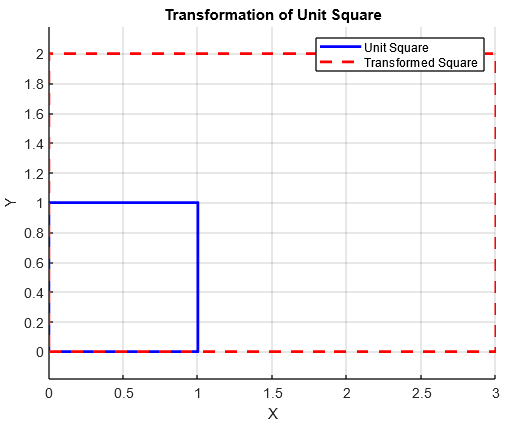
\includegraphics[width=1.00\textwidth]{complex_transformed_square.PNG}
  \label{fig3}
\end{figure}


\subsubsection*{Part e}

Operating with matrix $W$ as calculated above on the unit square $G$ yields:

\[ 
W' = W \cdot G = 
\begin{bmatrix}
    w_{11}g_{11} + w_{12}g_{21} & w_{11}g_{12} + w_{12}g_{22} & w_{11}g_{13} + w_{12}g_{23} & w_{11}g_{14} + w_{12}g_{24} \\
    w_{21}g_{11} + w_{22}g_{21} & w_{21}g_{12} + w_{22}g_{22} & w_{21}g_{13} + w_{22}g_{23} & w_{21}g_{14} + w_{22}g_{24}
\end{bmatrix}
\]

\[W' = 
\begin{bmatrix}
    0 & 3 & 3 & 0 \\
    0 & 0 & 2 & 2 \\
\end{bmatrix}
\]

Since $G$ was a unit square this will have the same form as the matrix in problem 4d.

\subsection*{Problem 5}

The figure shows three outline versions of the letter F. The second one is obtained from the first by shrinking horizontally by a factor of 0.75, and the third is obtained from the first by shearing horizontally by a factor of 0.25

\subsubsection*{Part a}

The data matrix for the letter F can be expressed using the matrix $D$:

\[
  D =
  \left[ {\begin{array}{ccccccccccc}
    0 & 1 & 1 & 4 & 4 & 1 & 1 & 6 & 6 & 0 & 0\\
    0 & 0 & 4 & 4 & 5 & 5 & 7 & 7 & 8 & 8 & 0\\
  \end{array} } \right]
\]

Depicted below:
\begin{figure}[H]
  \centering
  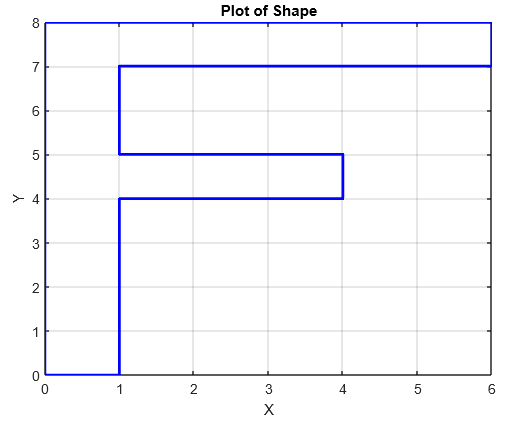
\includegraphics[width=1.00\textwidth]{letter_f.PNG}
  \label{fig3}
\end{figure}


\subsubsection*{Part b}

The transformed matrix is $F'$. This matrix is the result of horizontally shrinking the letter F by a factor of 0.75. This corresponds to the transformed matrix:

\[
  F' =
  \left[ {\begin{array}{ccccccccccc}
    0 & 0.75 & 0.75 & 3 & 3 & 0.75 & 0.75 & 4 & 4 & 0 & 0\\
    0 & 0 & 4 & 4 & 5 & 5 & 7 & 7 & 8 & 8 & 0\\
  \end{array} } \right]
\]

This matrix is obtained by multiplying D by a matrix T. This matrix is:

\[T = 
\begin{bmatrix}
    0.75 & 0 \\
    0 & 1\\
\end{bmatrix}
\]

\subsubsection*{Part c}

The transformed matrix is $F'$. This matrix is the result by shearing the letter F by a factor of 0.25. This shear matrix is:

Shear matrix with a factor of 0.25:
\[
  S =
  \left[ {\begin{array}{cc}
    1 & 0.25 \\
    0 & 1 \\
  \end{array} } \right]
\]

Resultant matrix after shear transformation:

\[
  DS =
  \left[ {\begin{array}{ccccccccccc}
    0 & 1 & 2 & 5 & 5.25 & 2.25 & 2.75 & 7.75 & 8 & 2 & 0\\
    0 & 0 & 4 & 4 & 5 & 5 & 7 & 7 & 8 & 8 & 0\\
  \end{array} } \right]
\]

\subsection*{Problem 6}

\[
  D =
  \left[ {\begin{array}{cccccc}
    0 & 1 & 2 & 1 & 0 & 0\\
    0 & 0 & 2 & 4 & 4 & 0\\
  \end{array} } \right]
\]

\subsubsection*{Part a}

\subsubsection*{Part b}

T is the matrix:

\[
  T =
  \left[ {\begin{array}{cc}
    1 & 1 \\
    0 & -1 \\
  \end{array} } \right]
\]

Acting with this matrix on matrix D produces:

\[
  TD =
  \left[ {\begin{array}{cccccc}
    0 & 1 & 4 & 5 & 4 & 0\\
    0 & 0 & -2 & -4 & -4 & 0\\
  \end{array} } \right]
\]

This produces a reflection across the x-axis in addition to a shear by 1 towards the positive x-direction as depicted below:

\begin{figure}[H]
  \centering
  \includegraphics[width=0.45\textwidth]{problem6b_figure.PNG}
  \label{fig3}
\end{figure}


\subsubsection*{Part c}

To express matrix $T$ as the product of a shear matrix and a reflection matrix, we recall that a reflection
matrix across the x-axis can be expressed as:

\[
  R =
  \left[ {\begin{array}{cc}
    1 & 0 \\
    0 & -1 \\
  \end{array} } \right]
\]

While a shear matrix can be expressed for this problem as:

\[
  S =
  \left[ {\begin{array}{cc}
    1 & -1 \\
    0 & 1 \\
  \end{array} } \right]
\]

Multiplying these two matrices yields the matrix $T$:

\[
  T = SR= 
  \left[ {\begin{array}{cc}
    1 & 0 \\
    0 & -1 \\
  \end{array} } \right]
\]

\pagebreak

\title{Computer Graphics - Project II}
\author{Erica Cain, Takiya Eastmond, Makayla Greer, Twymun Safford}
\date{February 20th, 2024}

\begin{titlingpage}
    \begin{center}
        \vspace*{3cm}
        {\Huge \thetitle}\\[0.5cm]
        {\Large \theauthor}\\[2cm]
        {\large \thedate}
    \end{center}
\end{titlingpage}


\section*{Projects 1 - Computer Graphics II}

\subsection*{Problem 1}

Use a rotation matrix to find the new coordinates of the given point when it is rotated through the given angle.

\subsubsection*{Part a}

The point $P$ can be represented in vector form as: 

\[
  P= 
  \left[ {\begin{array}{c}
    1 \\
    4 \\
  \end{array} } \right]
\]

The 2D rotation matrix for an angle $\theta$ is given by:
\[
\begin{bmatrix}
\cos \theta & -\sin \theta \\
\sin \theta & \cos \theta
\end{bmatrix}
\]

When $\theta$ = $\frac{\pi}{2}$, this rotation matrix becomes:

\[
\begin{bmatrix}
0 & -1 \\
1 & 0
\end{bmatrix}
\]

Operating with this rotation matrix on the vector yields:


\[P ' =
\begin{bmatrix}
0 & -1 \\
1 & 0
\end{bmatrix}
*   \left[ {\begin{array}{c}
    1 \\
    4 \\
  \end{array} } \right]
\]

Which yields:

\[
  P'= 
  \left[ {\begin{array}{c}
    -4 \\
    1 \\
  \end{array} } \right]
\]


\subsubsection*{Part b}

The point $P$ can be represented in vector form as: 

\[
  P= 
  \left[ {\begin{array}{c}
    -2 \\
    1 \\
  \end{array} } \right]
\]

The 2D rotation matrix for an angle $\theta$ is given by:
\[
\begin{bmatrix}
\cos \theta & -\sin \theta \\
\sin \theta & \cos \theta
\end{bmatrix}
\]


When $\theta$ = $\frac{\pi}{3}$, this rotation matrix becomes:

\[
\begin{bmatrix}
\frac{1}{2} & -\frac{\sqrt{3}}{2} \\
\frac{\sqrt{3}}{2} & \frac{1}{2}
\end{bmatrix}
\]

Operating with this rotation matrix on the vector yields:


\[P ' =
\begin{bmatrix}
\frac{1}{2} & -\frac{\sqrt{3}}{2} \\
\frac{\sqrt{3}}{2} & \frac{1}{2}
\end{bmatrix}
\left[ {\begin{array}{c}
    -2 \\
     1 \\
  \end{array} } \right]
\]

Which yields:

\[
  P'= 
  \left[ {\begin{array}{c}
    -1 - \frac{\sqrt{3}}{2} \\
    \frac{1}{2} - \sqrt{3} \\
  \end{array} } \right]
\]


\subsubsection*{Part c}

The point $P$ can be represented in vector form as: 

\[
  P= 
  \left[ {\begin{array}{c}
    -2 \\
    -2 \\
  \end{array} } \right]
\]

The 2D rotation matrix for an angle $\theta$ is given by:
\[
\begin{bmatrix}
\cos \theta & -\sin \theta \\
\sin \theta & \cos \theta
\end{bmatrix}
\]

When $\theta$ = $\frac{5\pi}{4}$, this rotation matrix becomes:

\[
\begin{bmatrix}
-\frac{\sqrt{2}}{2} & -\frac{\sqrt{2}}{2} \\
\frac{\sqrt{2}}{2} & -\frac{\sqrt{2}}{2}
\end{bmatrix}
\]

Operating with this rotation matrix on the vector yields:


\[P ' =
\begin{bmatrix}
-\frac{\sqrt{2}}{2} & -\frac{\sqrt{2}}{2} \\
\frac{\sqrt{2}}{2} & -\frac{\sqrt{2}}{2}
\end{bmatrix}
\left[ {\begin{array}{c}
    -2 \\
    -2 \\
  \end{array} } \right]
\]

Which yields:

\[
  P'= 
  \left[ {\begin{array}{c}
    2 \sqrt{2} \\
    0 \\
  \end{array} } \right]
\]

\subsubsection*{Part d}

The point $P$ can be represented in vector form as: 

\[
  P= 
  \left[ {\begin{array}{c}
    7 \\
    3 \\
  \end{array} } \right]
\]

The 2D rotation matrix for an angle $\theta$ is given by:
\[
\begin{bmatrix}
\cos \theta & -\sin \theta \\
\sin \theta & \cos \theta
\end{bmatrix}
\]

When the angle is negative, this matrix becomes:

\[
\begin{bmatrix}
\cos \theta & \sin \theta \\
-\sin \theta & \cos \theta
\end{bmatrix}
\]



When $\theta$ = -$\frac{\pi}{3}$, this rotation matrix becomes:

\[
\begin{bmatrix}
\frac{1}{2} & \frac{\sqrt{3}}{2} \\
-\frac{\sqrt{3}}{2} & \frac{1}{2}
\end{bmatrix}
\]

Operating with this rotation matrix on the vector yields:


\[P ' =
\begin{bmatrix}
\frac{1}{2} & \frac{\sqrt{3}}{2} \\
-\frac{\sqrt{3}}{2} & \frac{1}{2}
\end{bmatrix}
\left[ {\begin{array}{c}
    7 \\
    3 \\
  \end{array} } \right]
\]

Which yields:

\[
  P'= 
  \left[ {\begin{array}{c}
    \frac{7 + 3\sqrt{3}}{2} \\
    \frac{3 - 7\sqrt{3}}{2} \\
  \end{array} } \right]
\]

\subsection*{Problem 2}

The original shape (arrow) is depicted below:

\begin{figure}[H]
  \centering
  \includegraphics[width=0.45\textwidth]{arrow.PNG}
  \label{fig3}
\end{figure}

\subsubsection*{Part a}

The data matrix for this arrow is:

\[
  D =
  \left[ {\begin{array}{cccccccc}
    1 & 2 & 2 & 3 & 2 & 2 & 1 & 1\\
    2 & 2 & 1 & 2.5 & 4 & 3 & 3 & 2\\
  \end{array} } \right]
\]

The 2D rotation matrix for an angle $\theta$ is given by:
\[
\begin{bmatrix}
\cos \theta & -\sin \theta \\
\sin \theta & \cos \theta
\end{bmatrix}
\]


When $\theta$ = $\frac{2\pi}{3}$ like in this problem, this rotation matrix becomes:

\[
\begin{bmatrix}
-\frac{1}{2} & -\frac{\sqrt{3}}{2} \\
\frac{\sqrt{3}}{2} & -\frac{1}{2}
\end{bmatrix}
\]

If we act with this rotation matrix on the arrow (based on points), this yields:

\[
  D' = RD =
  \begin{bmatrix}
   -\frac{1}{2} & -\frac{\sqrt{3}}{2} \\
   \frac{\sqrt{3}}{2} & -\frac{1}{2}
\end{bmatrix}
  \left[ {\begin{array}{cccccccc}
    1 & 2 & 2 & 3 & 2 & 2 & 1 & 1\\
    2 & 2 & 1 & 2.5 & 4 & 3 & 3 & 2\\
  \end{array} } \right]
\]

Which yields the final shape of our matrix (and our arrow's points after rotation) as:

\[
  D' =
  \left[ {\begin{array}{cccccccc}
    -2.23 & -2.73 & -1.87 & -3.67 & -4.46 & -3.69 & -3.10 & -2.23\\
    -0.13 & 0.73 & 1.23 & 1.35 & -0.27 & 0.23 & -0.63 & -0.13\\
  \end{array} } \right]
\]

This now looks like:



\subsection*{Problem 3}

Sketch the image represented by the data matrix $D$:

\[
  D =
  \left[ {\begin{array}{ccccccccc}
    2 & 3 & 3 & 4 & 4 & 1 & 1 & 2 & 2\\
    1 & 1 & 3 & 3 & 4 & 4 & 3 & 3 & 1\\
  \end{array} } \right]
\]

Sketched image is:

\begin{figure}[H]
  \centering
  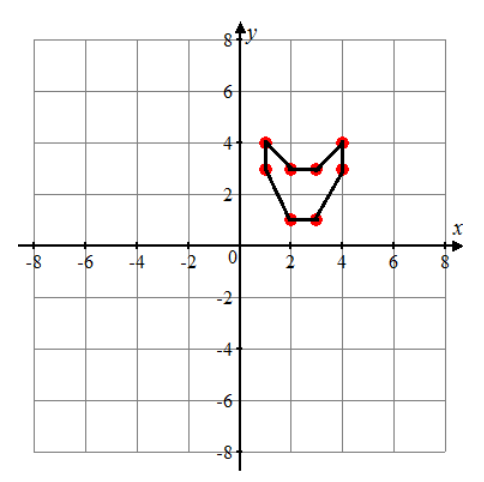
\includegraphics[width=1.0\textwidth]{plot_unique_shape.PNG}
  \label{fig3}
\end{figure}

The 2D rotation matrix for an angle $\theta$ is given by:
\[
\begin{bmatrix}
\cos \theta & -\sin \theta \\
\sin \theta & \cos \theta
\end{bmatrix}
\]

When $\theta$ = $\frac{\pi}{4}$, this rotation matrix becomes:

\[
\begin{bmatrix}
\frac{\sqrt{2}}{2} & -\frac{\sqrt{2}}{2} \\
\frac{\sqrt{2}}{2} & \frac{\sqrt{2}}{2}
\end{bmatrix}
\] 

The transformation matrix that is an expansion by a factor of 2 in the x-direction is:

\[T = 
\begin{bmatrix}
2 & 0 \\
0 & 1
\end{bmatrix}
\] 

The matrix RT which results from multiplying matrix $T$ by matrix $R$ yields:

\begin{align*}
RT=\begin{bmatrix}
\frac{\sqrt{2}}{2} & -\frac{\sqrt{2}}{2} \\
\frac{\sqrt{2}}{2} & \frac{\sqrt{2}}{2}
\end{bmatrix}
\times
\begin{bmatrix}
2 & 0 \\
0 & 1
\end{bmatrix}
&=
\begin{bmatrix}
\frac{\sqrt{2}}{2} \times 2 + (-\frac{\sqrt{2}}{2}) \times 0 & \frac{\sqrt{2}}{2} \times 0 + (-\frac{\sqrt{2}}{2}) \times 1 \\
\frac{\sqrt{2}}{2} \times 2 + \frac{\sqrt{2}}{2} \times 0 & \frac{\sqrt{2}}{2} \times 0 + \frac{\sqrt{2}}{2} \times 1
\end{bmatrix} \\
&=
\begin{bmatrix}
\sqrt{2} & -\frac{\sqrt{2}}{2} \\
\sqrt{2} & \frac{\sqrt{2}}{2}
\end{bmatrix}
\end{align*}

Sketch of RT:

\begin{figure}[H]
  \centering
  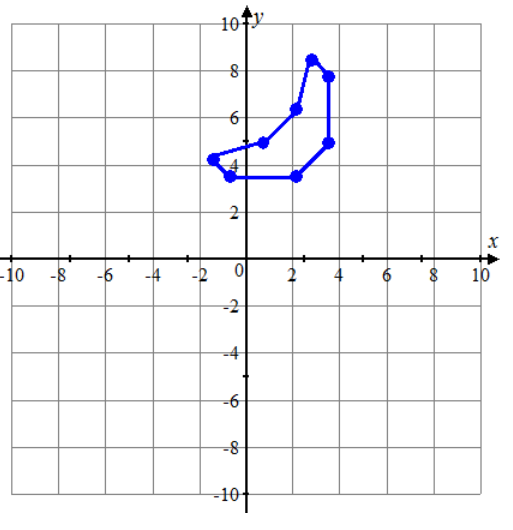
\includegraphics[width=0.45\textwidth]{sketch_of_rt.PNG}
  \label{fig3}
\end{figure}


While matrix TR which results from multiplying matrix $R$ by matrix $T$ yields:

\[
TR = 
\begin{pmatrix}
2 \times \frac{\sqrt{2}}{2} + 0 \times \frac{\sqrt{2}}{2} & 2 \times (-\frac{\sqrt{2}}{2}) + 0 \times \frac{\sqrt{2}}{2} \\
0 \times \frac{\sqrt{2}}{2} + 1 \times \frac{\sqrt{2}}{2} & 0 \times (-\frac{\sqrt{2}}{2}) + 1 \times \frac{\sqrt{2}}{2}
\end{pmatrix}
\]

This simplifies to
\[
TR = 
\begin{pmatrix}
\sqrt{2} & -\sqrt{2} \\
\frac{\sqrt{2}}{2} & \frac{\sqrt{2}}{2}
\end{pmatrix}
\]

The matrix product $TRD$ will be:

\[
TRD = 
\begin{pmatrix}
2 & 0 \\
0 & 1
\end{pmatrix}
\begin{pmatrix}
\frac{\sqrt{2}}{2} & -\frac{\sqrt{2}}{2} \\
\frac{\sqrt{2}}{2} & \frac{\sqrt{2}}{2}
\end{pmatrix}
\begin{pmatrix}
2 & 3 & 3 & 4 & 4 & 1 & 1 & 2 & 2 \\
1 & 1 & 3 & 3 & 4 & 4 & 3 & 3 & 1
\end{pmatrix}
\]

\[
TRD = 
\begin{pmatrix}
\sqrt{2} & -\sqrt{2} \\
\frac{\sqrt{2}}{2} & \frac{\sqrt{2}}{2}
\end{pmatrix}
\begin{pmatrix}
2 & 3 & 3 & 4 & 4 & 1 & 1 & 2 & 2 \\
1 & 1 & 3 & 3 & 4 & 4 & 3 & 3 & 1
\end{pmatrix}
\]

While the matrix product $RTD$ yields:

\[
  RTD =
\begin{bmatrix}
\sqrt{2} & -\frac{\sqrt{2}}{2} \\
\sqrt{2} & \frac{\sqrt{2}}{2}
\end{bmatrix}
\begin{pmatrix}
2 & 3 & 3 & 4 & 4 & 1 & 1 & 2 & 2 \\
1 & 1 & 3 & 3 & 4 & 4 & 3 & 3 & 1
\end{pmatrix}
\]


\subsection*{Problem 4}

Let $R$ be the rotation matrix for the angle $\theta$. We want to show that $R^{-1}$ is the rotation matrix for the angle $-\theta$.

The inverse of a rotation matrix is the transpose of the matrix, thus:

\[
R^{-1} = R^T
\]

To show that $R^{-1}$ is the rotation matrix for the angle $-\theta$, we need to show that $(R^{-1})^T$ represents a rotation of $-\theta$.

\[
(R^{-1})^T = (R^T)^T = R
\]

Since $R$ is the rotation matrix for the angle $\theta$, $R$ represents a rotation of $\theta$. Therefore, $(R^{-1})^T = R$ represents a rotation of $\theta$, which is the same as the original matrix $R$. 

Thus, $R^{-1}$ is the rotation matrix for the angle $-\theta$.

This can be proven explicitly. Using trig. identities, we know that $cos(-\theta)$ = $cos(\theta)$
and that $sin(-\theta)$ = -$sin(\theta)$ as depicted below:

\[
\begin{bmatrix}
\cos \theta & \sin \theta \\
-\sin \theta & \cos \theta
\end{bmatrix}
\]

\subsection*{Problem 5}
\[
(x, y) \leftrightarrow 
  \left[ {\begin{array}{c}
    x\\
    y\\
    1\\    
  \end{array} } \right]
\],
\[
  T =
  \left[ {\begin{array}{ccc}
    1 & 0 & h\\
    0 & 1 & k\\
    0 & 0 & 1\\
  \end{array} } \right]
\]

\subsubsection*{Problem 5a}

Show that matrix $T$ translates the point (x,y)  to the point (x+h, y+h) by verifying the following matrix
multiplication.

\[
  P' =
  \left[ {\begin{array}{ccc}
    1 & 0 & h\\
    0 & 1 & k\\
    0 & 0 & 1\\
  \end{array} } \right]
\left[ {\begin{array}{c}
    x\\
    y\\
    1\\    
  \end{array} } \right]  
\]

The result is:

\[
\begin{bmatrix}
    1 \cdot x + 0 \cdot y + h \cdot 1 \\
    0 \cdot x + 1 \cdot y + k \cdot 1 \\
    0 \cdot x + 0 \cdot y + 1 \cdot 1 \\
\end{bmatrix}
=
\begin{bmatrix}
    x + h \\
    y + k \\
    1 \\
\end{bmatrix}
\]

\subsubsection*{Problem 5b}

The inverse of the matrix \( T \) is given by:
\[
T^{-1} =
\left[ \begin{array}{ccc}
1 & 0 & -h \\
0 & 1 & -k \\
0 & 0 & 1 \\
\end{array} \right]
\]

By multiplying this matrix on the original point:

\[
\left[ \begin{array}{ccc}
1 & 0 & -h \\
0 & 1 & -k \\
0 & 0 & 1 \\
\end{array} \right]
\left[ \begin{array}{c}
x \\
y \\
1 \\
\end{array} \right]
=
\left[ \begin{array}{c}
1 \cdot x + 0 \cdot y + (-h) \cdot 1 \\
0 \cdot x + 1 \cdot y + (-k) \cdot 1 \\
0 \cdot x + 0 \cdot y + 1 \cdot 1 \\
\end{array} \right]
=
\left[ \begin{array}{c}
x - h \\
y - k \\
1 \\
\end{array} \right]
\]

We see that this will translate the point from (x,y) to (x-h, y-k).

\subsubsection*{Problem 5c}

\[
  P= 
\left[ {\begin{array}{c}
    x\\
    y\\
    1\\    
  \end{array} } \right]  
\]

Reflection in x-axis produces:

\[
  \begin{bmatrix}
    1 & 0 & 0 \\
    0 & -1 & 0 \\
    0 & 0 & 1 \\
  \end{bmatrix}
  \cdot
  \begin{bmatrix}
    x \\
    y \\
    1 \\
  \end{bmatrix}
  = 
  \begin{bmatrix}
    x \\
    -y \\
    1 \\
  \end{bmatrix}
\]


Expansion (or contraction) in x-direction produces:

\[
  \begin{bmatrix}
    c & 0 & 0 \\
    0 & 1 & 0 \\
    0 & 0 & 1 \\
  \end{bmatrix}
  \cdot
  \begin{bmatrix}
    x \\
    y \\
    1 \\
  \end{bmatrix}
  = 
  \begin{bmatrix}
    cx \\
    y \\
    1 \\
  \end{bmatrix}
\]

Shear in x-direction produces:

\[
  \begin{bmatrix}
    1 & c & 0 \\
    0 & 1 & 0 \\
    0 & 0 & 1 \\
  \end{bmatrix}
  \cdot
  \begin{bmatrix}
    x \\
    y \\
    1 \\
  \end{bmatrix}
  = 
  \begin{bmatrix}
    x + cy \\
    y \\
    1 \\
  \end{bmatrix}
\]

Rotation about the origin by angle $\theta$:

\[
  \begin{bmatrix}
    \cos(\theta) & -\sin(\theta) & 0 \\
    \sin(\theta) & \cos(\theta) & 0 \\
    0 & 0 & 1 \\
  \end{bmatrix} \cdot
  \begin{bmatrix}
    x \\
    y \\
    1 \\
  \end{bmatrix}
  = 
  \begin{bmatrix}
    x \cdot \cos(\theta) - y \cdot \sin(\theta) \\
    x \cdot \sin(\theta) + y \cdot \cos(\theta) \\
    1 \\
  \end{bmatrix}
\]

\subsubsection*{Problem 5d}

Sketch the image represented (in homogeneous coordinates) by this data matrix:

\begin{figure}[H]
  \centering
  \includegraphics[width=1.2\textwidth]{problem_5d.PNG}
  \label{fig3}
\end{figure}


The data matrix for the letter F can be expressed using the matrix $D$:

\[
  D =
  \left[ {\begin{array}{ccccccccccccc}
3 & 5 & 5 & 7 & 7 & 9 & 9 & 7 & 7 & 5 & 5 & 3 & 3 \\
7 & 7 & 5 & 5 & 7 & 7 & 9 & 9 & 11 & 11 & 9 & 9 & 7 \\
1 & 1 & 1 & 1 & 1 & 1 & 1 & 1 & 1 & 1 & 1 & 1 & 1 \\
  \end{array} } \right]
\]

\begin{figure}[H]
  \centering
  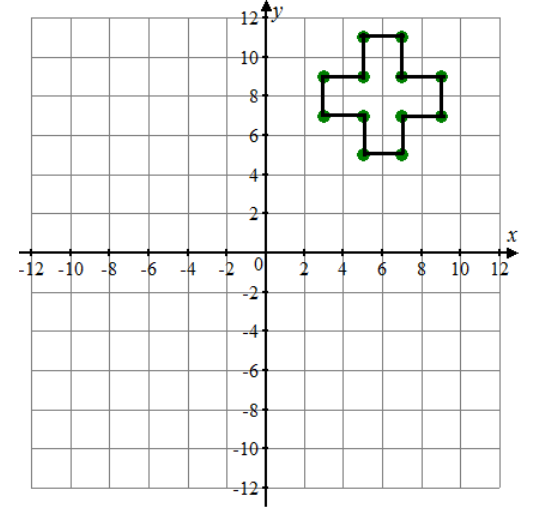
\includegraphics[width=1.2\textwidth]{cross.PNG}
  \label{fig3}
\end{figure}


The matrix that translates the image (based on the data matrix) 6 units left and 8 units down is:

\[
  \begin{bmatrix}
    1 & 0 & -6 \\
    0 & 1 & -8 \\
    0 & 0 & 1 \\
  \end{bmatrix}
\]

Multiplying the data matrix by the translation matrix produces:
\[
  TD =
  \begin{bmatrix}
    1 & 0 & -6 \\
    0 & 1 & -8 \\
    0 & 0 & 1 \\
  \end{bmatrix}
  \left[ {\begin{array}{ccccccccccccc}
3 & 5 & 5 & 7 & 7 & 9 & 9 & 7 & 7 & 5 & 5 & 3 & 3 \\
7 & 7 & 5 & 5 & 7 & 7 & 9 & 9 & 11 & 11 & 9 & 9 & 7 \\
1 & 1 & 1 & 1 & 1 & 1 & 1 & 1 & 1 & 1 & 1 & 1 & 1 \\
  \end{array} } \right]
\]

Which produces:

\begin{figure}[H]
  \centering
  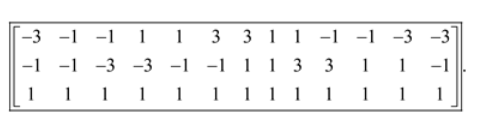
\includegraphics[width=1.0\textwidth]{matrix_5d_td.PNG}
  \label{fig3}
\end{figure}

The rotation matrix is: 
\[
  \begin{bmatrix}
    \cos(\theta) & -\sin(\theta) & 0 \\
    \sin(\theta) & \cos(\theta) & 0 \\
    0 & 0 & 1 \\
  \end{bmatrix}
\]

And for 45 degrees this matrix is:

\[
  \begin{bmatrix}
    \frac{\sqrt{2}}{2} & -\frac{\sqrt{2}}{2} & 0 \\
    \frac{\sqrt{2}}{2} & \frac{\sqrt{2}}{2} & 0 \\
    0 & 0 & 1 \\
  \end{bmatrix}
\]

The product of this rotation matrix with the prior matrix TD yields:

\begin{figure}[H]
  \centering
  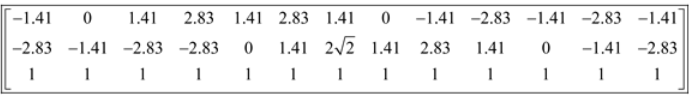
\includegraphics[width=1.0\textwidth]{matrix_5d_td2.PNG}
  \label{fig3}
\end{figure}

When multiplied by matrix $T$, an image will be translated 6 points left and 8 points down.

When multiplied by $RT$, an image will be translated 6 points left and 8 points down and rotated 45 degrees.

When multiplied by $T^{-1}RT$, an image will be translated 6 points left and 8 points down and rotated 45 degrees, but will then be moved back to the original place it started at. 



\pagebreak

\title{Image Manipulations}
\author{Erica Cain, Takiya Eastmond, Makayla Greer, Twymun Safford}
\date{February 20th, 2024}


\begin{titlingpage}
    \begin{center}
        \vspace*{3cm}
        {\Huge \thetitle}\\[0.5cm]
        {\Large \theauthor}\\[2cm]
        {\large \thedate}
    \end{center}
\end{titlingpage}

\section*{Original Image}

\begin{figure}[H]
  \centering
  
\includegraphics[width=1.00\textwidth]{tyler-hall.jpeg}
  \label{fig3}
\end{figure}

Code for the image manipulations are in the project subfolder "Matlab codes". Corresponding
matrices for manipulation are saved in the subfolder "Matrices". 

\section*{Image Manipulation - Reflection of Image (x- and y-axis)}

\subsection*{y-axis}

\begin{figure}[H]
  \centering
  
\includegraphics[width=1.00\textwidth]{tyler_hall_reflected_y.jpeg}
  \label{fig3}
\end{figure}

\subsection*{x-axis}

\begin{figure}[H]
  \centering
  
\includegraphics[width=1.00\textwidth]{tyler-hall-reflected-x.jpg}
  \label{fig3}
\end{figure}


\section*{Image Manipulation - Expansion}

\begin{figure}[H]
  \centering
  
\includegraphics[width=1.00\textwidth]{tyler-hall-expanded.jpeg}
  \label{fig3}
\end{figure}

\section*{Image Manipulation - Shear of Image (Factor of 0.75)}

\begin{figure}[H]
  \centering
  
\includegraphics[width=1.00\textwidth]{tyler-hall-sheared.jpeg}
  \label{fig3}
\end{figure}


\section*{Image Manipulation - Rotation of Image (67.36 degrees counterclockwise)}

\begin{figure}[H]
  \centering
  
\includegraphics[width=1.00\textwidth]{tyler-hall-rotated.jpeg}
  \label{fig3}
\end{figure}

\end{document}

